\documentclass[../synthesis.tex]{subfiles}
\graphicspath{{\subfix{../../../../images/}}}
\begin{document}
    The co-precipitation method\cite{a8} is a commonly used technique for the synthesis of nanophosphors, including 
    those intended for thermoluminescence dosimetry. This method involves the simultaneous precipitation of 
    metal cations and anions from a solution, resulting in the formation of nanocrystalline particles.
    The co-precipitation method offers advantages such as simplicity, cost-effectiveness, and scalability for 
    the synthesis of nanophosphors. However, careful control of reaction conditions and post-treatment steps 
    is essential to achieve desired particle properties and optimize the dosimetric performance of the 
    nanophosphors for thermoluminescence dosimetry applications. Here is an overview of the co-precipitation 
    method shown in\ref{fig:CoPrecipitationFlow}:
    \begin{Figure}
        \centering
        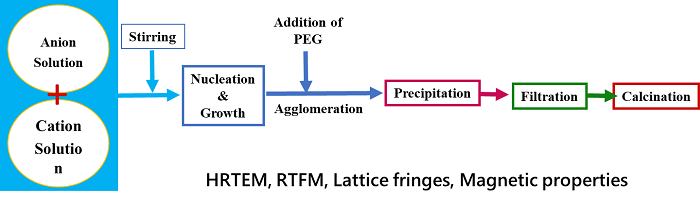
\includegraphics[width=0.8\linewidth]{CoPrecipitationFlow.png}
        \captionof{figure}{Synthesis using Co-Precipitation Method\cite{a7}}\label{fig:CoPrecipitationFlow}
    \end{Figure}
    \begin{itemize}
        \item \textbf{Selection of Precursor Salts:} Choose appropriate precursor salts that contain the 
        desired metal cations and anions for the nanophosphor composition. The choice of precursors depends on 
        the specific material being synthesized.
        \item \textbf{Preparation of Precursor Solution: } Dissolve the precursor salts in a suitable solvent 
        to prepare a precursor solution. The solvent should facilitate the dissolution of the precursors and 
        promote homogeneous mixing.
        \item \textbf{Control of Reaction Conditions: }Adjust the reaction conditions, including temperature, 
        pH, and reaction time, to control the nucleation and growth of the nanophosphor particles. The 
        reaction conditions play a crucial role in determining the size, composition, and crystallinity of the 
        resulting nanophosphors.
        \item \textbf{Precipitating Agent Addition: }Add a precipitating agent to the precursor solution to 
        induce the formation of the nanophosphor particles. The choice of precipitating agent depends on the 
        specific reaction system and desired properties of the nanophosphors. Commonly used precipitating 
        agents include ammonium hydroxide ($NH_4OH$), sodium hydroxide ($NaOH$), or carbonate solutions.
        \item \textbf{Precipitation and Aging: }Upon the addition of the precipitating agent, the metal 
        cations and anions react to form insoluble salts, resulting in the precipitation of nanocrystalline 
        particles. Allow the precipitates to age for a certain period, typically through continuous stirring 
        or aging at a specific temperature, to promote particle growth and improve crystallinity.
        \item \textbf{Filtration and Washing: }Separate the formed nanophosphor precipitates from the solution 
        by filtration. Wash the precipitates multiple times with a suitable solvent or deionized water to 
        remove any residual impurities or unreacted ions.
        \item \textbf{Drying and Calcination:} Dry the filtered nanophosphor precipitates at a controlled 
        temperature to remove the solvent and residual moisture. Depending on the specific material, the dried 
        precipitates may undergo a subsequent calcination process to enhance crystallinity and remove any 
        remaining organic species.
    \end{itemize}
    \begin{Figure}
        \centering
        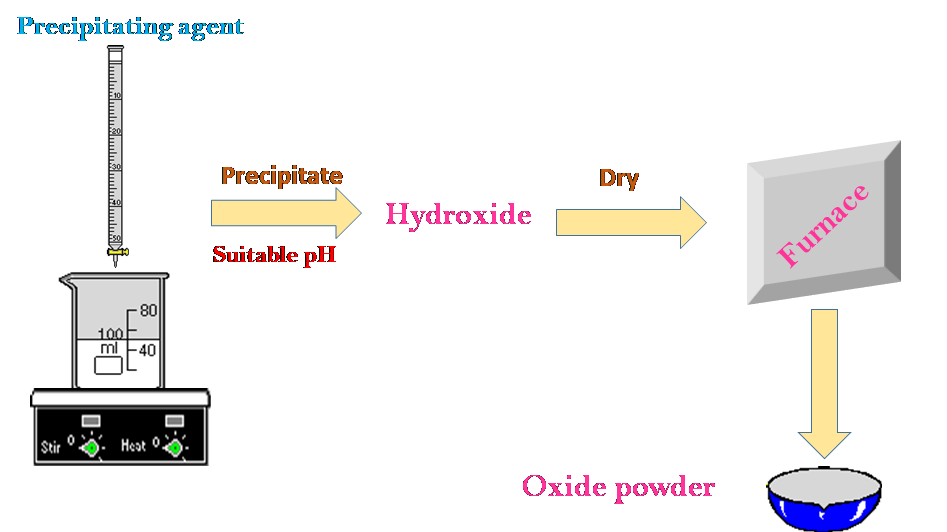
\includegraphics[width=0.8\linewidth]{CoPrecipitation.png}
        \captionof{figure}{Schematic diagram for Co-Precipitation Method\cite{u7}}\label{fig:CoPrecipitation}
    \end{Figure}
\end{document}